\chapter{Introduction}
\label{chap:intro}

Nowadays, technology is a fundamental part of our daily lives, as it facilitates solving problems that humans face as well as analyze data they can not easily interpret.
In the world of martial arts, there is no easy accurate way to study and analyze the performance of a trainee statistically. This absence of analysis is due to the lack of tools presented to the trainers and trainees.

\section{Aim of this project}
The aim of this project is to deliver an easy-to-use interface that displays training sessions' info and statistics. This in turn will help the trainers to get an accurate analysis of the trainee's performance and examine different aspects of a training session. This interface will allow multiple plugins to be to be plugged in simultaneously.

\section{Background}
In this project a multi-sensor tracking and analysis tool will be implemented. This tool would be connected to multiple plugins and sensors to record and analyze a specific physical workout routine to track performance and fitness level of a practitioner over a single or multiple sessions.

\begin{figure}[htbp]
\centering 
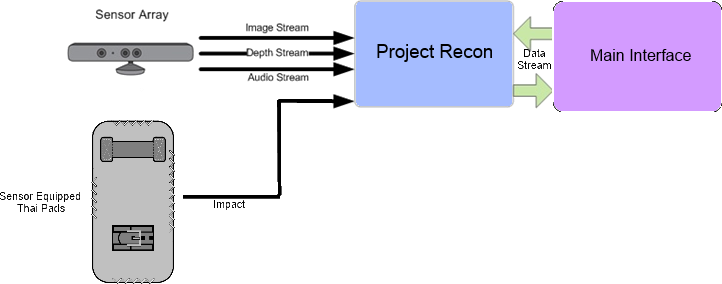
\includegraphics[width=1.0\linewidth]{General.png} 
\caption{General Overview} 
\label{fig:overview} 
\end{figure} 

This interface itself is very generic that any type of plugins could be connected to it (check \ref{sec:installation} for configuration steps)\footnote{The plugin should have the ability to send the data to the main interface through sockets.}.
